\documentclass[conference]{style/IEEEtran}  
\IEEEoverridecommandlockouts
% The preceding line is only needed to identify funding in the first footnote. If that is unneeded, please comment it out.
\usepackage{cite}
\usepackage{amsmath,amssymb,amsfonts}
\usepackage{algorithmic}
\usepackage[dvipdfmx]{graphicx,color}
\usepackage{textcomp}
\usepackage{xcolor}

\def\BibTeX{{\rm B\kern-.05em{\sc i\kern-.025em b}\kern-.08em
    T\kern-.1667em\lower.7ex\hbox{E}\kern-.125emX}}

\usepackage{bm}

%% \usepackage{geometry}
%% \usepackage[dvipdfmx]{graphicx}
%% \usepackage{booktabs}
%% \usepackage[dvipdfmx]{color}
%% \usepackage{amsmath,amssymb}
%% \usepackage{url}
%% \usepackage{listings,jlisting}
%% \usepackage{here}
%% \usepackage[dvipdfmx]{hyperref}


%% \usepackage{ascmac}

%% \geometry{
%%   left=15mm,
%%   top=15mm,
%%   right=15mm,
%%   bottom=15mm
%%  }
%% %
%% \renewcommand{\lstlistingname}{コード}
%% %


%
\begin{document}

\title{test title}
\author{
  No Name
  
}

\maketitle
%% \section{Introduction}\label{section:intro}

%% テンプレートです。
hoge\cite{bib:HELMHOLTZ_FURUSHO_EN}

\begin{figure}[tbp]   
  \centering   
  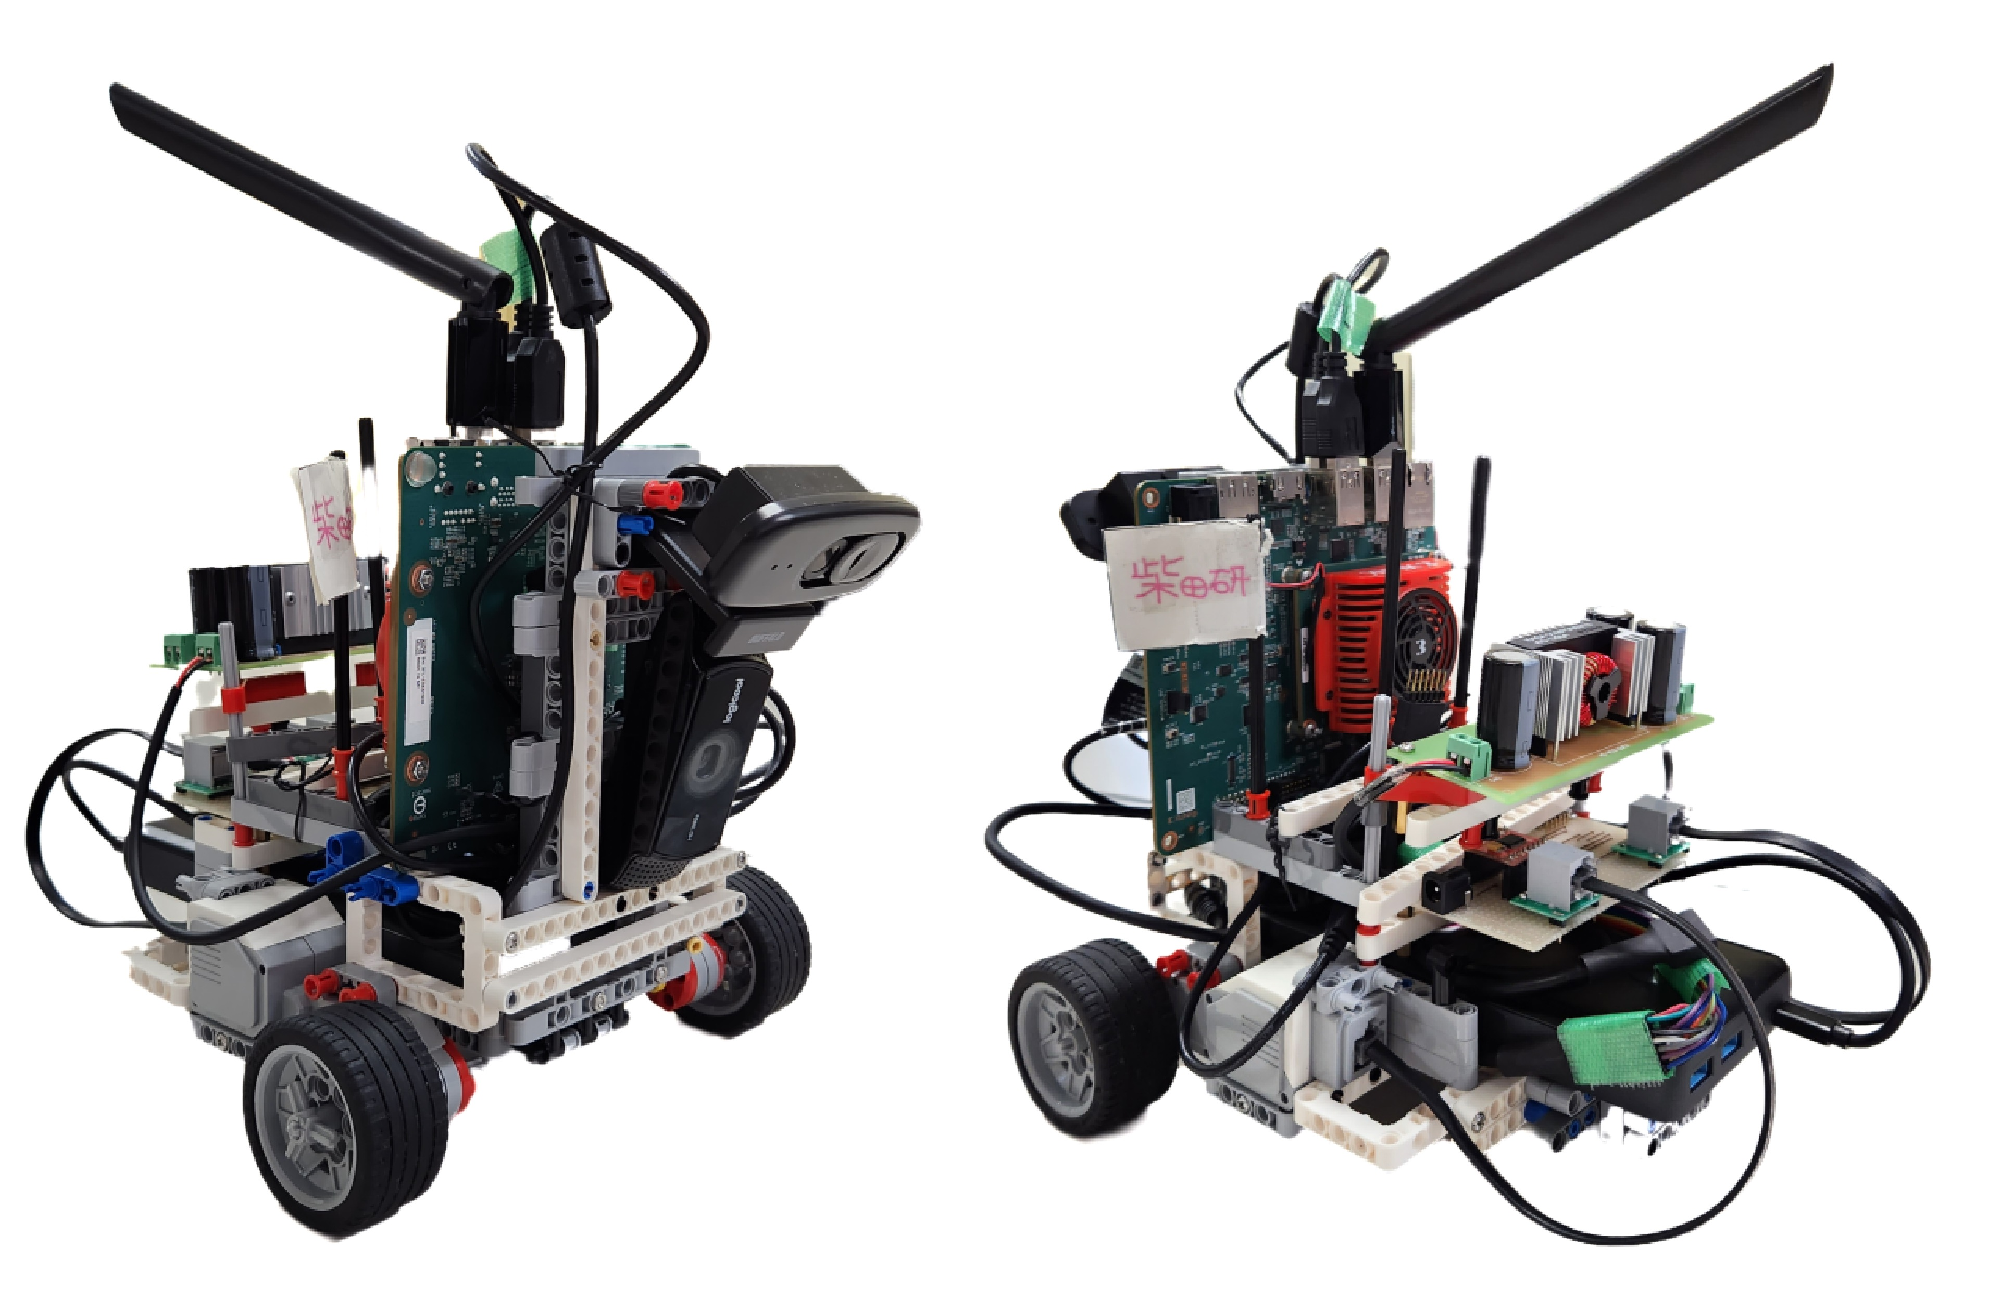
\includegraphics[width=0.48\textwidth]{img/template.pdf}
  \caption{overview}
  \label{fig:template}
\end{figure}                                                                                                             
                 


\section{Intoroduction}\label{section:intro}
%% \cite{bib:neck_surgery}\cite{bib:reconstructive_microsurgery}.

In recent surgical procedures, there is a surgical technique called microsurgery,
in which delicate operations such as dissection and union of blood vessels and nerves are performed using loupes and microscopic cameras.

%% このマイクロサージェリーは前述のとおり繊細な手術であることから,執刀医の手の不随意な振動である振戦が手術の妨げになっている.また,振戦を意識しながらの手術は執刀医に大きな負担がかかる.
%% そのため,執刀医の振戦を抑制するシステムの導入により,安全性の向上や執刀医の負担の軽減が期待される

Because microsurgery is a delicate procedure, as mentioned above, the involuntary vibration of the primary surgeon's hand, tremor, interferes with the operation.
Surgery while being aware of the tremor places a heavy burden on the primary surgeon.
Therefore, the introduction of a system that suppresses the tremor of the primary surgeon is expected to improve safety and reduce the burden on the primary surgeon.
\cite{bib:Adaptive_cancelling}\cite{bib:Design_and_Validation}.



%% 振戦を抑制する手法として,振戦の振動成分を抽出し逆位相の振動を手術器具に加えて抑制する手法が考えられる.
%% しかし,振戦抽出のために加速度センサ等を手術器具の先端や執刀医の手元に取り付けることは繊細な手術の妨げとなる可能性があり,センサを用いた振戦抽出は望ましくない.
%% また,執刀医の意図的な操作を妨げることのないように抽出した振動に対するフィルタリング機構が必要である.
%% しかし,逆位相の振動による振戦抑制を行うためには逆位相の振動の位相遅れを最小限にする必要があるため,通常のバンドパスフィルタは適さない.

One possible method to suppress tremor is to extract the vibration component of the tremor and apply vibration in the opposite phase to the surgical instrument to suppress it.
However, the use of accelerometers or other sensors attached to the tips of surgical instruments or to the surgeon's hands for tremor extraction may interfere with delicate surgical procedures,
and sensor-based tremor extraction is not desirable.
In addition, a filtering mechanism for the extracted vibration is necessary so as not to interfere with the primary surgeon's intentional manipulation.
However, to suppress tremor caused by vibrations in opposite phase, the phase delay of vibrations in opposite phase must be minimized, making an ordinary band-pass filter unsuitable.


%% そこで眞邉らは,顕微鏡カメラより入力される動画像からリアルタイムに振戦の振動成分を抽出するシステムを提案し, 
%% FPGAへ実装した\cite{bib:Image-Based_Vibration_Extraction}.
 %% 眞邉らが提案したシステムは,動画像から特徴量マッチングを用いてオプティカルフローを推定し,位相遅れのない適応フィルタである
 %% BMFLC(Bandlimited Multiple Fourier Linear Combiner)\cite{bib:BMFLC}
 %% を用いてフィルタリングを行い,振戦の振動成分を抽出する.
 %% しかし,眞邉らの提案システムは実機動作するシステムの定量的評価や,実際に抽出した振戦の逆位相の振動を出力する加振装置と接続しての抑制実験は行われていない.

Therefore, Manabe et al. proposed a system to extract vibration components of a tremor in real time from a video image input from a microscope camera, and implemented the system in an FPGA.\cite{bib:Image-Based_Vibration_Extraction}
The system proposed by Manabe et al. estimates the optical flow from the video image using feature matching,
filters it using BMFLC (Bandlimited Multiple Fourier Linear Combiner)\cite{bib:BMFLC},
an adaptive filter with no phase delay, and extracts the vibration components of the tremor.
The vibration component of the tremor is extracted. However, the system proposed by Manabe et al. has not been quantitatively evaluated in actual operation,
nor have suppression experiments been conducted by connecting the system to a shaker that actually outputs vibration in the opposite phase of the extracted tremor.

 
 %% そこで本研究では,眞邉らが提案した実機動作する振動抽出FPGAシステムの定量的評価と,
 %% 振戦の抑制実験を行ってのシステムの有効性を示すことを目的とする.


The purpose of this study is to quantitatively evaluate the vibration extraction FPGA system proposed by Manabe et al.
and to demonstrate the effectiveness of the system by conducting experiments to suppress tremors.
 
%% システムの定量的評価を行うためには振動成分の真値がわかる動画像をシステムに入力し,システムの出力を真値と比較する必要がある.


%% \section{関連研究}\label{section:research}
%% 振動抽出FPGAシステムの評価を行うために様々な関連研究が行われている.
%% 本節では,振戦抑制システムの評価のための関連研究について述べる.

%%   山下らは, SoC FPGAを用いてリアルタイム画像処理システムを定量的に評価するための検証プラットフォームを構築した\cite{bib:kensyo}.
%% %%   この検証プラットフォームは,実機動作する
%% %% FPGA画像処理システムに対してリアルタイムな検証用動画像の入力とそれに対する出力値の取得を可能にし,
%% %% この出力値から実機動作するFPGA画像処理システムの定量的評価を行える検証環境である.
%% 山下らの検証プラットフォームはSoC FPGAによるPS-PL通信を用いることでPL部に実装された実機動作する
%% FPGA画像処理システムに対してリアルタイムな検証用動画像の入力とそれに対する出力値の取得を可能にし,
%% この出力値から実機動作するFPGA画像処理システムの定量的評価を行える検証環境である.
%% %% PS部ではUbuntu OSをブートさせており,ファイルシステムの利用やネットワーク接続など,
%% %% より柔軟に評価を行うことができる.
%% この検証環境を使用することにより,検証対象システムに大きな変更を加えることなく,
%% 最小限の手順で画像処理システムの定量的評価を行うことが可能である.

  
  
%% 中央大学では,磁気式3次元位置測定システムのVIPER\cite{bib:VIPER}とBMFLC-KF (BMFLC-Kalman Filter)\cite{bib:BMFLC-KF}と呼ばれる適応推定フィルタを用いて手術器具先端の振戦を検出し,
%% 逆位相の振動をリニアアクチュエータを用いて手術器具先端に加振して振戦を抑制するハンドヘルド型の振動抑制装置を開発した.
%% %% 日根らが開発した振戦抑制装置の構成を図\ref{figure:tremor_suppression_config}に示す.
%% 振戦抑制装置は,ハンドヘルド部に手術器具を挿入し,内蔵されている  %% マイクロコンピュータであるTeensy4.0\cite{bib:Teensy4.0}等で構成される逆位相波発生装置を用いて
%% 逆位相波発生装置を用いて
%% 手術器具先端の振動の逆位相の振動を加振することで,振戦による器具先端の振動を抑制する.
%% しかし,この振動推定の手法は手術器具先端にマイクロセンサを取り付ける必要があるため,実際の手術に用いることはできない.
%% %% \begin{figure}[tb]
%% %%   \centering
%% %%   \includegraphics[width = 6cm]{img/environment/tremor_suppression_config.png}
%% %%   \caption{振戦抑制装置の構成}
%% %%   \label{figure:tremor_suppression_config}
%% %% \end{figure}

%% 田中らは,手術器具の模型をヒトが手に持った際の手術器具先端の水平方向の振戦を含む振動を測定し,測定した振動を高精度に再現する振戦再現装置を開発した\cite{bib:tremor_reproduction}.
%% %% 田中らが開発した振戦再現装置の構成を図\ref{figure:tremor_reproduction_config}に示す.
%% 振戦再現装置は,事前にVIPERを用いて測定した手術器具をヒトが保持した際の模型器具先端の振動を再現する.
%% %% \begin{figure}[tb]
%% %%   \centering
%% %%   \includegraphics[width = 6cm]{img/environment/tremor_reproduction_config.png}
%% %%   \caption{振戦再現装置の構成}
%% %%   \label{figure:tremor_reproduction_config}
%% %% \end{figure}




%%  %% そこで本研究では,田中らが開発した振戦再現装置と山下らの検証プラットフォームを用いて,眞邉らが提案した振戦抽出システムの定量的評価を行う.
%%  %% また,振戦抽出システムと日根らの振戦抑制装置内部の加振システムを接続するためのインタフェースを作成し,振戦抽出システムが抽出した振戦の振動の逆位相の振動を手術器具先端に加振する
%%  %% 振戦の抑制テストを行い,システムの有効性を示す.


%%  %% 本稿の構成は以下の通りである.まず,第2章で本研究の背景や目的を述べる.
%%  %% 第3章では,本研究で利用するFPGAや,評価対象であるリアルタイム振戦抽出システムの概要について述べる.
%%  %% 第4章では,振戦検出システムの評価の際に利用する評価環境について述べる.
%%  %% 第5章では,振戦抽出システムの評価について述べ,最後に,第6章で本研究の結論を述べる.

\section{Real-time vibration extraction system}\label{section:system}
%% 本節では,評価対象である眞邉らの振動抽出FPGAシステムの概要について述べる.

In this section, we provide an overview of the Real-time vibration extraction system of Manabe et al.

\subsection{Gradient Calculation}\label{subsection:gradient}
%% まずはじめに、入力グレースケール画像を平滑化した画像の勾配$l_x$,$l_y$から、
%% 勾配角$\theta$が計算される。フレームバッファのメモリリソースを節約するため、
%% $\theta$は1,2または3ビットに量子化される。$\theta$は以下の式で計算される。:

First, the gradient angle $\theta$ is calculated from the gradients $l_x$ and $l_y$
of the smoothed input grayscale image. To save memory resources in the frame buffer,
$\theta$ is quantized to 1, 2 or 3 bits. The $\theta$ is computed by the following equation :


\begin{equation}
  \label{equ:grad_angle1}
  \theta_3(x,y) = \left\lfloor \frac{4 \times {\rm atan2}(I_y(x,y),I_x(x,y))}{\pi} \right\rfloor\mod 8
  \end{equation}

\begin{equation}
  \label{equ:grad_angle2}
  \theta(x,y) = \left\lfloor \frac{\theta_3(x,y) + e(x,y)}{2^{3-Q}} \right\rfloor
\end{equation}

\begin{equation}
  \label{equ:grad_angle3}
  e(x,y) = (x+y)\mod 2^{3-Q}
  \end{equation}

%% $Q\in{1,2,3}$は量子化ビット幅、eはオフセットである.
where $Q\in{1,2,3}$ is the quantization bit-width and e is the offset.



\subsection{Feature Calculation}\label{subsection:feature}

%% 先ほど算出した$\theta$から特徴量を算出する.特徴量には,照明変化に剛健で回転不変性の
%% あるRI-HOG(Rotation-Invariant Histogram of Oriented Gradient)\cite{bib:RHOG}
%% をベースにしたものを使用する.
Calculate the features from the $\theta$ calculated earlier.
The features are based on RIHOG (Rotation-Invariant Histogram of Oriented Gradient),
which is rigid and rotationally invariant to illumination changes.
To make the feature rotationally invariant,

%% 量子化された$\theta$を復号し、3ビットの勾配角$\theta'$を算出する:

%% \begin{equation}
%%   \label{equ:theta_dash}
%%   \theta'(x,y) = (2^{3-Q} \theta(x,y)-e(x,y)) \mod 8
%% \end{equation}

%% 特徴量を回転不変にするために、ピクセルを囲む$C \times C$の領域(セル)内
%% の3ビットの相対勾配角をセル内の各ピクセルに対して求め、
%% セル内の相対勾配角のヒストグラムを作成することで、簡略化されたRIHOG特徴量が計算されます。
%% 相対勾配角が$i(0 i 7)$であるピクセルの数を$ni$とすると、特徴記述子$H$は次のように表されます:
a simplified RIHOG feature is computed by finding the 3-bit relative gradient angle
in the $C \times C$ region (cell) surrounding the pixel for each pixel
in the cell and creating a histogram of the relative gradient angles in the cell.
Let $ni$ be the number of pixels whose relative gradient angle is $i(0 \leq i \leq 7)$,
then the feature descriptor $H$ is expressed as follows:

\begin{align}
  \label{equation:equ_RIHOG}
  H(x,y) = (n_0,n_1,n_2,...,n_7)^T \\
  \left(  0 \leq n_i \leq C^2 -1 , \sum_{i=0}^{7}n_i = C^2 -1  \right) \notag
\end{align}



\subsection{Optical Flow Estimation Using Feature Matching}\label{label:estimation}

%% 現在のフレームの特徴量$H_k$と前のフレームの特徴量$K_{k-1}$をもとに、
%% パターンマッチを用いて各ピクセルのオプティカルフローを求める。
%% 点$(x,y)$におけるオプティカルフローが$F(x,y)$である場合、$(x,y)$は前のフレーム
%% $(x-y,y-v)$に相当する。
%% ヒストグラム交差(HI)を用いて類似度$S(u,v)$を求め,
%% 探索窓の中から$S(u,v)$が最大になる$(u,v)$の探索を行う。
%% $S(u,v)$は次のように求められる:


Based on the feature $H_k$ of the current frame and the feature $K_{k-1}$ of the previous frame,
the optical flow of each pixel is obtained using pattern matching.
If the optical flow at point $(x,y)$ is $F(x,y)$,
then $(x,y)$ corresponds to the previous frame $(x-y,y-v)$.
Calculate the similarity $S(u,v)$ using histogram intersection (HI)
and search for $(u,v)$ in the search window where $S(u,v)$ is the largest.
The $S(u,v)$ is obtained as follows:


\begin{equation}
  \label{equ:similarity}
  S(u,v) = \max(S_{raw}(u,v)-p(u,v),0)
\end{equation}

\begin{equation}
  \label{equ:similarity2}
  S_{raw}(u,v) = HI(H_k(x,y),H_{k-1}(x-u,y-v))
\end{equation}

\begin{equation}
  \label{equ:similarity3}
  p(u,v)=\left\lfloor \frac{\sqrt{u^2+v^2}}{2} + 0.5 \right\rfloor
\end{equation}


%% ヒストグラム$H_1=(n_1,i)$、$H_2=(n_2,i)$のヒストグラム交差は次のように定義される。
The histogram intersection of histograms $H_1=(n_1,i)$ and $H_2=(n_2,i)$ is defined as follows:

\begin{equation}
  \label{equ:hist_intersection}
  (0 \leq HI \leq C),HI(H_1,H_2)=\sum_{i} \min(n_{1,i},n_{2,i}) 
\end{equation}


%% また、$F(x,y)$の信頼度$R(x,y)$を求める:
Also, find the confidence level $R(x,y)$ of $F(x,y)$:

\begin{equation}
  \label{equ:confidence}
  R(x,y) =  \max_{u,v} S(u,v) - \bar{S} 
\end{equation}

\begin{equation}
  \label{equ:mean_similarity}
  \bar{S} = \frac{\sum_{u,v}S(u,v)}{K^2}
\end{equation}

%% $R(x,y)$は平均類似度と最大類似度の差であり、特異的に類似度の高いフローを優先的に選ぶ役割を果たす。

The $R(x,y)$ is the difference between the mean similarity and maximum similarity and serves to preferentially select flows that are specifically similar.


\subsection{Block-Mean-Optical FLow Calculation}\label{subsection:block-optical}

%% 次に、画像を$B \times B$のサイズのちいさなブロックに分割し、各ブロックのオプティカルフローの平均を求める。
%% $i$ブロックの中の$j$番目のピクセルのオプティカルフロー$F_i(j)=(u_ij,v_ij)$と信頼度$R_i(j)$
%% から、以下のように計算する:


Next, divide the image into tiny blocks of size $B \times B$ and find the average optical flow
of each block From the optical flow $F_i(j)=(u_ij,v_ij)$ of the $j$th pixel
in the $i$ block and the confidence level $R_i(j)$,
calculate The following is calculated as follows:

\begin{equation}
  \label{equ:block_opt}
   \bar F_i=(\bar u_i,\bar v_i)=
   \left(   \frac{ \sum_ju_{ij} \times R_i(j) }{\sum_jR_i(j)} , \frac{ \sum_jv_{ij} \times R_i(j) }{\sum_jR_i(j)} \right)
\end{equation}


\subsection{BMFLC Filtering}\label{subsection:BMFLC_filtering}

%% 求めた各ブロックの平均オプティカルフローに対して,BMFLCによるフィルタリングを独立に行う.
%% BMFLCは,通過周波数帯$[f_{\mathit{lower}},f_{\mathit{upper}}]$を等間隔で$L$個
%% のサブバンドに分割し,現在の時刻$t[\rm{sec}]$によって定まる
%% 参照入力ベクトル$\bm{x}$を以下のように求める.


The average optical flow of each block is independently filtered by BMFLC,
which divides the passband $[f_{\mathit{lower}},f_{\mathit{upper}}]$ into
$L$ subbands at equal intervals, with the current time $t[\rm{sec}]$,
and the reference input vector $\bm{x}$ determined
by the current time $t[{\rm{sec}}]$ is obtained as follows:

\begin{align}
  \label{equ:Vector}
  & \bm{x} = (\sin \omega_0t,\ldots,\sin \omega_{L-1}t,
  \cos \omega_0t,\ldots,cos \omega_{L-1}t)^T \\
  &  \left(
  \omega_r=2\pi \left( f_{\mathit{lower}} +
  \frac{f_{\mathit{upper}}-f_{\mathit{lower}}}{L}r \right)
  \right)
\end{align}
  

   
%% BMFLCの通過周波数帯は振戦の特徴を考慮し$8\sim12$ Hzとしている.
%% ブロック$i$の水平及び垂直方向の適応重みベクトルを$\bm{w}_{x,i},\bm{w}_{y,i}$とすると,ブロック$i$の平均オプティカルフロー$\bar F'_i=(\bar u'_i,\bar v'_i)$は以下によって得られる:


The pass frequency band of the BMFLC is set to $8^sim12$ Hz, considering the characteristics of the tremor.
Let $\bm{w}_{x,i},\bm{w}_{y,i}$ be the horizontal and vertical adaptive weight vectors of block $i$,
the mean optical flow $\bar F'_i=(\bar u'_i,\bar v'_i)$ of block $i$ is obtained by:


\begin{equation}
  \label{equ:}
  \bar F'_i=(\bar u'_i,\bar v'_i) = (\bm{w}_{x,i}^T\bm{x} , \bm{w}_{y,i}^T\bm{x})
\end{equation}


 
%% また,ブロック$i$が指定した周波数帯域の振動をどの程度含んでいるかを示すブロック重み$W_i$を式\eqref{equation:equ16}より求める.

The block weight $W_i$, which indicates the degree
to which block $i$ contains vibrations in the specified frequency band,
is obtained from the equation\eqref{equation:equ16}.


 
 \begin{equation}
   \label{equation:equ16}
   W_i = \max \left(
   \frac{ \|\bm{w}_{x,i}\|^1 + \|\bm{w}_{y,i}\|^1 }{2} - \tau ,0
   \right)
   \end{equation}


 %% ここで,$\tau$は重みの値が一定値を下回るブロックを無視するための閾値である.
 %% 適応重みベクトルの更新は以下のように行われる.
 where $\tau$ is a threshold for ignoring blocks whose weights are below a certain value.
 The update of the adaptive weight vector is performed as follows:
 
\begin{align}
  &\bm{w}_{x,i} \leftarrow
  \bm{w}_{x,i} + 2\mu(\bar u_i - \bar u'_i)\bm{x} \\
  &\bm{w}_{y,i} \leftarrow
  \bm{w}_{y,i} + 2\mu(\bar v_i - \bar v'_i)\bm{x}
\end{align}

%% $\mu$はゲインパラメータであり,収束の速度と安定のバランスを
%% 保つ役割がある.

$mu$ is a gain parameter and serves to balance the speed and stability of convergence.
 
%% 最後に,振動成分$(\Delta x , \Delta y)$を以下のように求める.
Finally, the vibration component $(\Delta x , \Delta y)$ is obtained as follows:

 \begin{equation}
   \label{equation:equ17}
   (\Delta x , \Delta y) = \left(
   \frac{\sum_i ( \bar u'_i \times W_i )}{\sum_i W_i} , \frac{\sum_i ( \bar v'_i \times W_i )}{\sum_i W_i}
   \right)
 \end{equation}

 %% これがシステムの最終的な出力である.
 This is the final output of the system.



%% \bibliographystyle{jplain}
\bibliographystyle{style/IEEEtran.bst}
%% \bibliography{bib/0-refs.bib}
\bibliography{bib/99-refs.bib}

\end{document}
